\documentclass{article}
\usepackage[utf8]{inputenc}
\usepackage{listings}
\usepackage{float}
\usepackage{graphicx}

\usepackage{color}
 
\definecolor{codegreen}{rgb}{0,0.6,0}
\definecolor{codegray}{rgb}{0.5,0.5,0.5}
\definecolor{codepurple}{rgb}{0.58,0,0.82}
\definecolor{backcolour}{rgb}{0.95,0.95,0.92}
 
\lstdefinestyle{mystyle}{
    backgroundcolor=\color{backcolour},   
    commentstyle=\color{codegreen},
    keywordstyle=\color{magenta},
    numberstyle=\tiny\color{codegray},
    stringstyle=\color{codepurple},
    basicstyle=\footnotesize,
    breakatwhitespace=false,         
    breaklines=true,                 
    captionpos=b,                    
    keepspaces=true,                 
    numbers=left,                    
    numbersep=5pt,                  
    showspaces=false,                
    showstringspaces=false,
    showtabs=false,                  
    tabsize=2,
    language=python
}
\lstset{style=mystyle}


\title{Tugas Pemrograman Section 4}
\author{Ahmad Agung Tawakkal\\
        1184015\\
        D4 TI 1B}
\date{November 2019}

\graphicspath{{figure/}}

\begin{document}

\maketitle

\newpage


\section{Teori}
    \subsection{Apa itu fungsi file CSV, jelaskan sejarah dan contoh}
        \begin{itemize}
            \item Fungsi file CSV
                \paragraph{}Format file csv \textit{Comma Separated Values} yaitu suatu format data pada basis data dimana setiap record yang dapat dipisahkan dengan menggunakan tanda koma (`,’) atau juga bisa dengan menggunakan titik koma (`;’) sebagai tanda pemisah antara datu elemen dengan elemen yang lainnya. Selain bahasa programnya yang sederhana, format ini juga dapat dibuka dengan menggunakan berbagai \textit{text-editor} seperti Notepad, Wordpad, dan MS Excel.
            \item Sejarah file CSV
                \paragraph{} Nilai yang dipisahkan oleh koma adalah format data yang memberi tanggal lebih awal pada komputer pribadi lebih dari satu dekade: kompiler IBM Fortran (level H extended) di bawah OS / 360 mendukungnya pada tahun 1972. Input / output yang diarahkan oleh daftar ("bentuk bebas") didefinisikan dalam FORTRAN 77, disetujui pada tahun 1978. Input yang diarahkan daftar menggunakan koma atau spasi untuk pembatas, sehingga string karakter yang tidak dikutip tidak dapat mengandung koma atau spasi.
                \paragraph{}Nama (nilai dipisahkan koma) dan singkatan (CSV) digunakan pada tahun 1983. Manual untuk komputer Osborne Executive, yang menggabungkan SuperCalc spreadsheet, mendokumentasikan konvensi kutipan CSV yang memungkinkan string berisi koma yang disematkan, tetapi manual tersebut tidak menentukan konvensi untuk menyematkan tanda kutip dalam string yang dikutip. Daftar nilai yang dipisahkan koma lebih mudah untuk diketik (misalnya ke dalam kartu berlubang) daripada data yang selaras dengan kolom tetap dan cenderung menghasilkan hasil yang salah jika suatu nilai dilubangi satu kolom dari lokasi yang dituju.
                \paragraph{}Pada 2014 IETF menerbitkan RFC7111 yang menjelaskan aplikasi fragmen URI ke dokumen CSV. RFC7111 menentukan bagaimana rentang baris, kolom, dan sel dapat dipilih dari dokumen CSV menggunakan indeks posisi. Pada 2015 W3C, dalam upaya meningkatkan CSV dengan semantik formal, mempublikasikan draft rekomendasi pertama untuk standar metadata CSV, yang dimulai sebagai rekomendasi pada bulan Desember tahun yang sama.
            \newpage
            \item Contoh 
                \lstinputlisting[language=Python]{src/teori/praktikum.csv}
        \end{itemize}
    
    \subsection {Aplikasi-aplikasi yang bisa membuat file CSV}
        \begin{itemize}
            \item Text Editor (Notepad, Wordpad, dll)
            \item Spreadsheet (Microsoft Excel)
        \end{itemize}
        
    \subsection{Cara menulis dan membaca file CSV pada Excel}
        \begin{itemize}
            \item Membuka aplikasi excel
            \item K adalah kolom dan B adalah baris
            \item Kemudian K1 dan B1 di isi dengan Npm, K1 dan B2 di isi dengan Nama, K1 dan B2 di isi dengan Kelas
            \item Kemudian pada baris ke selanjutnya adalah ricord.
            \begin{figure}[ht]
                \centerline{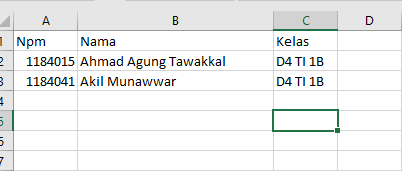
\includegraphics[width=10cm]{Capture.PNG}}
            \end{figure}
            \item Selanjutnya jika telah seperti atas maka selanjutnya kita save as dan pada save as type kita ganti jadi csv (Comman delimited)
            \newpage
            \begin{figure}[ht]
                \centerline{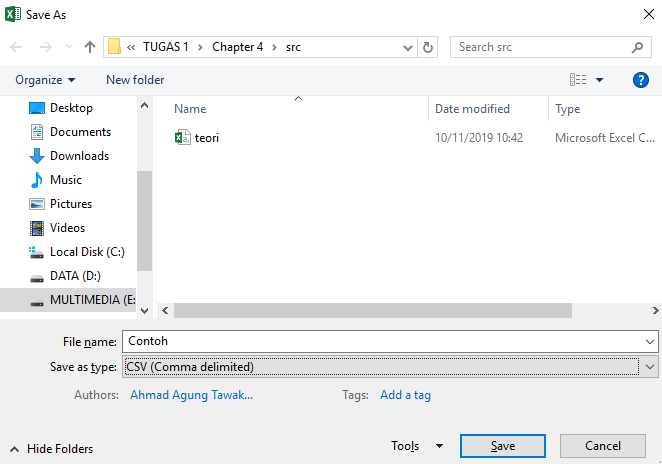
\includegraphics[width=10cm]{Capture1.PNG}}
            \end{figure}
            \item Maka akan file csv telah dibuat.
        \end{itemize}
    
    \subsection{Sejarah library CSV}
        \paragraph{} Format yang disebut CSV \textit{Comma Separated Values} adalah format impor dan ekspor paling umum untuk spreadsheet dan basis data. Format CSV digunakan selama bertahun-tahun sebelum upaya untuk menggambarkan format dengan cara standar di RFC 4180. Kurangnya standar yang didefinisikan dengan baik berarti bahwa perbedaan halus sering ada dalam data yang diproduksi dan dikonsumsi oleh aplikasi yang berbeda. Perbedaan-perbedaan ini dapat membuatnya menjengkelkan untuk memproses file CSV dari berbagai sumber.
        \paragraph{}Namun, sementara pembatas dan mengutip karakter bervariasi, format keseluruhan cukup mirip sehingga dimungkinkan untuk menulis satu modul yang dapat secara efisien memanipulasi data seperti itu, menyembunyikan detail membaca dan menulis data dari programmer. Modul csv mengimplementasikan kelas untuk membaca dan menulis data tabular dalam format CSV.
        
    \subsection{Sejarah library Pandas}
        \paragraph{}Pandas adalah toolkit yang powerfull sebagai alat analisis data dan struktur untuk bahasa pemrograman Python. Dengan menggunakan pandas kita dapat mengolah data dengan mudah, salah satu fiturnya adalah Dataframe. Dengan adanya fitur dataframe kita dapat membaca sebuah file dan menjadikannya tabble serta juga dapat mengolah suatu data dengan menggunakan operasi seperti join, distinct, group by, agregasi, dan lain-lain yang terdapat pada SQL. Banyak format file yang dapat dibaca menggunakan Pandas, seperti file .txt, .csv, .tsv dan lainnya. Agar lebih jelas mari kita mencobanya secara langsung.
    
    \subsection{Fungsi-fungsi yang terdpat pada library CSV}
        \begin{itemize}
            \item reader
                \paragraph{} Fungsi ini digunakan untuk membaca isi file berformat CSV dari list.
                \lstinputlisting[language=Python, caption =  Membaca file berformat CSV list., firstline=8, lastline=14]{src/teori/1184015.py}
            \item DictReader
                \paragraph{}  Fungsi ini digunakan untuk membaca isi file berformat CSV dari dictionary.
                \lstinputlisting[language=Python, caption =  Membaca file berformat CSV dictionary., firstline=16, lastline=22]{src/teori/1184015.py}
            \item write
                \paragraph{} Fungsi ini digunakan untuk menulis file berformat CSV dari list.
                \lstinputlisting[language=Python, caption =  Menulis file berformat CSV list., firstline=24, lastline=31]{src/teori/1184015.py}
            \newpage
            \item DictWrite
                \paragraph{}  Fungsi ini digunakan untuk menulis file berformat CSV dari dictionary.
                \lstinputlisting[language=Python, caption =  Menulis file berformat CSV dictionary., firstline=33, lastline=42]{src/teori/1184015.py}
        \end{itemize}
     
    \subsection{Fungsi-fungsi yang terdpat pada library Pandas}
        \begin{itemize}
            \item read\_csv
                \paragraph{} Fungsi ini digunakan untuk membaca isi file berformat CSV.
                \lstinputlisting[language=Python, caption =  Membaca file berformat CSV pandas., firstline=44, lastline=48]{src/teori/1184015.py}
            \item to\_csv
                \paragraph{} Fungsi ini digunakan untuk menulis file berformat CSV.
                \lstinputlisting[language=Python, caption =  Menulis file berformat CSV pandas., firstline=50, lastline=54]{src/teori/1184015.py}
        \end{itemize}
    \newpage
    \subsection{Bukti bebas plagialisme}
        \begin{figure}[ht]
            \centerline{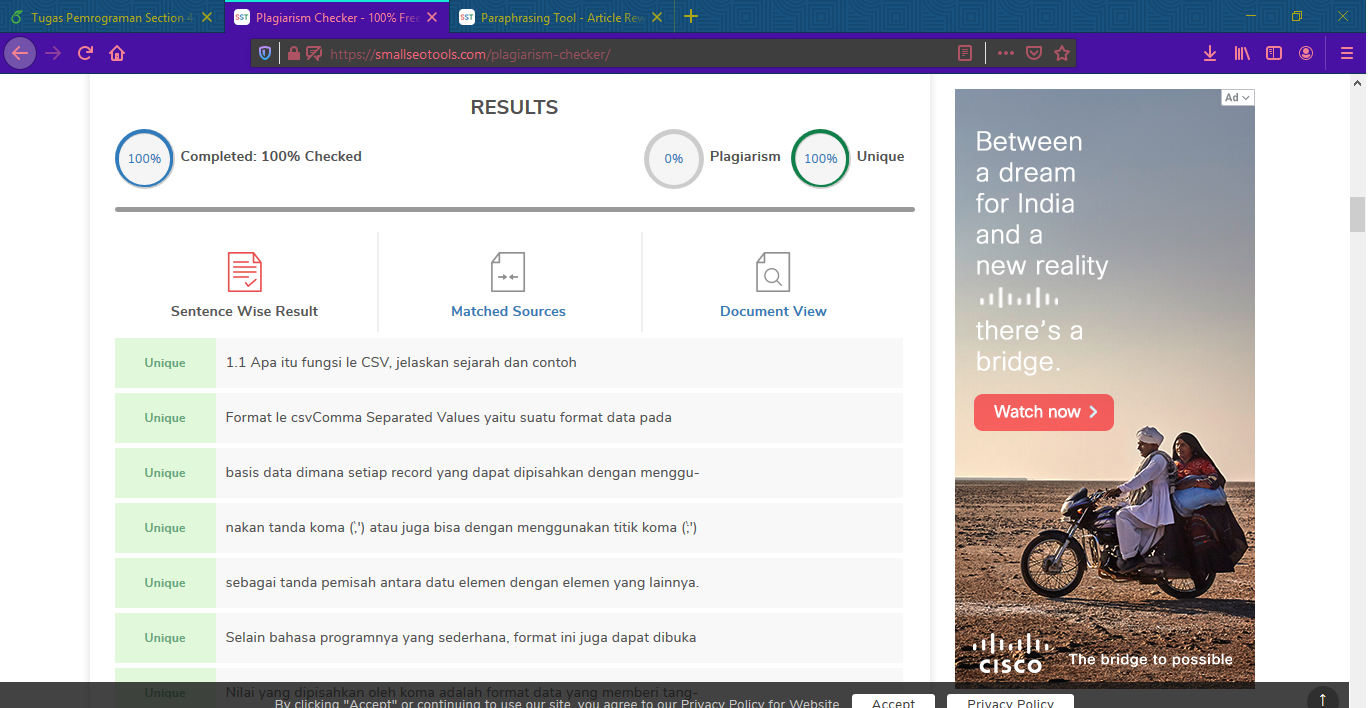
\includegraphics[width=10cm]{Capture2.PNG}}
        \end{figure}
    
\section{Keterampilan Pemrograman}
    \subsection*{Soal 1}
        \paragraph{}Membuat fungsi (file terpisah/library dengan nama NPM csv.py) untuk membuka file csv dengan lib csv mode list. Berikut adalah pemanggilan file csv dengan library csv yang menggunakan list.
        \lstinputlisting[language=Python, firstline=11, lastline=15]{src/keterampilan/1184015csv.py}
    
    \subsection*{Soal 2}
        \paragraph{}Membuat fungsi (file terpisah/library dengan nama NPM csv.py) untuk membuka file csv dengan lib csv mode dictionary. Berikut adalah pemanggilan file csv dengan library csv yang menggunakan dictionary.
        \lstinputlisting[language=Python, firstline=18, lastline=22]{src/keterampilan/1184015csv.py}
        
    \subsection*{Soal 3}
        \paragraph{}Membuat fungsi (file terpisah/library dengan nama NPM pandas.py) untuk membuka file csv dengan lib csv mode list. Berikut adalah pemanggilan file csv dengan library pandas yang menggunakan list.
        \lstinputlisting[language=Python, firstline=11, lastline=13]{src/keterampilan/1184015pandas.py}
        
    \subsection*{Soal 4}
        \paragraph{}Membuat fungsi (file terpisah/library dengan nama NPM pandas.py) untuk membuka file csv dengan lib csv mode dictionary. Berikut adalah pemanggilan file csv dengan library csv yang menggunakan dictionary.
        \lstinputlisting[language=Python, firstline=16, lastline=19]{src/keterampilan/1184015pandas.py}
        
    \subsection*{Soal 5}
        \paragraph{}Membuat fungsi pada file NPMpandas.py, untuk mengubah format tanggal menjadi standar dataframe. Berikut cara mengubah standar penulisan tanggal dengan mengikuti standar penulisan dari pandas.
        \lstinputlisting[language=Python, firstline=22, lastline=24]{src/keterampilan/1184015pandas.py}
    
    \subsection*{Soal 6}
        \paragraph{}Membuat fungsi pada file NPMpandas.py, untuk mengubah index kolom. Berikut muerpakan index kolom.
        \lstinputlisting[language=Python, firstline=27, lastline=30]{src/keterampilan/1184015pandas.py}
    
    \subsection*{Soal 7}
        \paragraph{}Membuat fungsi pada file NPMpandas.py, untuk mengubah atribut atau nama kolom berikut merupakan pengguna untuk mengubah nama atibut yang digunakan, atau merubah nama header.
        \lstinputlisting[language=Python, firstline=33, lastline=36]{src/keterampilan/1184015pandas.py}
        
    \subsection*{Soal 8}
        \paragraph{}Membuat program main.py untuk menggunakan library NPMcsv.py yang dapat membuat file dan membaca file csv.
        \lstinputlisting[language=Python, firstline=8, lastline=13]{src/keterampilan/main.py}
        
    \subsection*{Soal 9}
        \paragraph{}Membuat program main.py untuk menggunakan library NPMpandas.py yang dapat membuat file dan membaca file csv.
        \lstinputlisting[language=Python, firstline=16, lastline=21]{src/keterampilan/main.py}
        
    \subsection{Cek Plagialisme}
        \begin{figure}[ht]
            \centerline{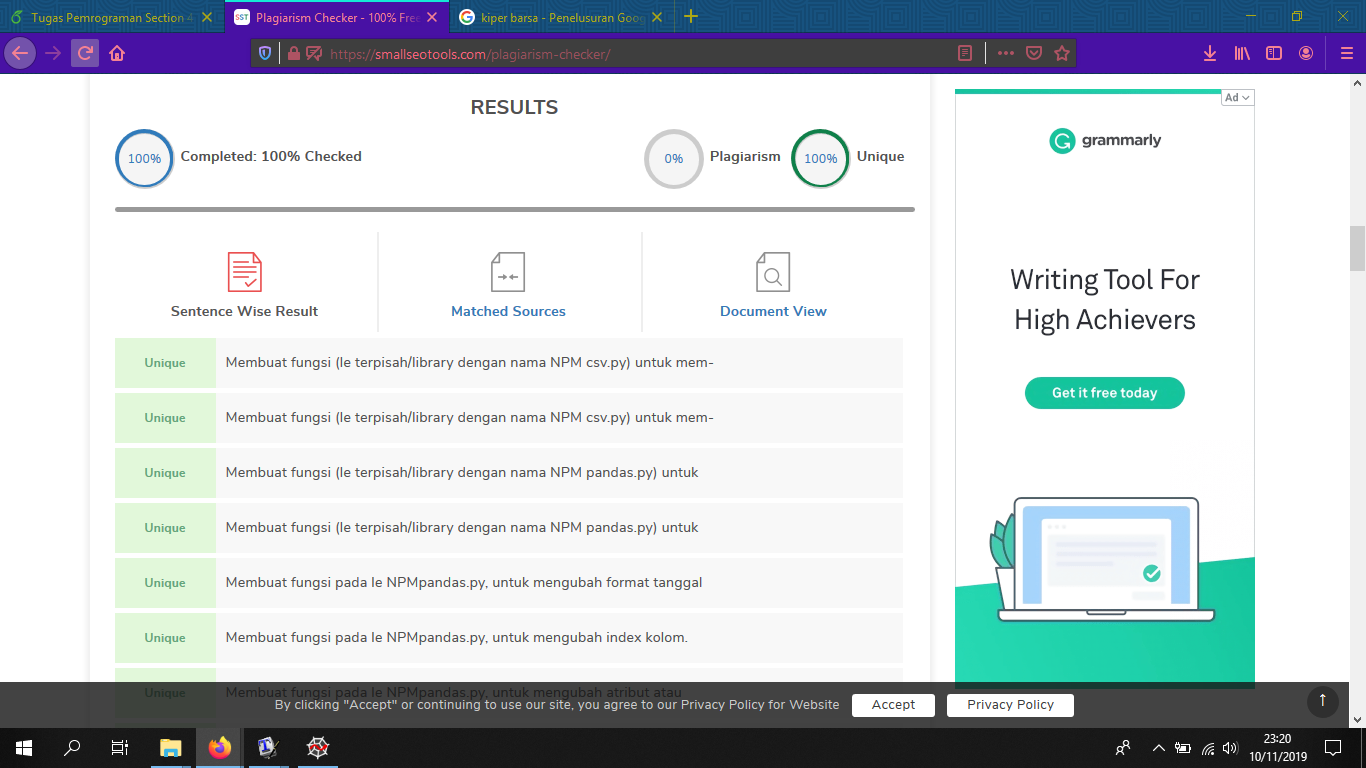
\includegraphics[width=10cm]{Capture3.PNG}}
        \end{figure}
\newpage
\section{Penanganan error}
    \paragraph{}Dalam menulis code program diperlukan keteilian agar program yang dibut tidak memilili error. Contoh mengunakan Try Except agar agar dapat memudahkan bagian yang error sebagai berikut.
    \lstinputlisting[language=Python, firstline=57, lastline=68]{src/keterampilan/1184015.py}

\section{Presentasi Tugas}
    \paragraph{}Link = 

\end{document}


